\documentclass[bibliography=numbered,listof=numbered,12pt,a4paper,openany,ngerman,plainfootsepline,plainheadsepline]{scrbook}
% Change "article" to "report" to get rid of page number on title page
\usepackage{amsmath,amsfonts,amsthm,amssymb}
\usepackage{setspace}

% Definitionen f�r Tabellen
\usepackage{Tabbing}
\usepackage{multirow}
\usepackage{latexsym,amssymb}
\usepackage{colortbl}
\usepackage[margin=1in,headsep=2.5cm]{geometry}
\usepackage{colortbl}

%define own color for Tables
\definecolor{mygrey}{rgb}{0.411765,0.411765,0.411765}
\definecolor{darkgrey}{rgb}{0.8,0.8,0.8}
\definecolor{hellgrau}{rgb}{0.95,0.95,0.95}




\usepackage{lastpage}
\usepackage{cite}
\usepackage{tocbasic}
\usepackage[automark,						%Automatische Kopfzeile
						%headtopline,				%Linie �ber dem Seitenkopf
						%plainheadtopline,	%Plain, Linie �ber dem Seitenkopf
						headsepline,				%Linie zwischen Kopf und Textk�rper
						%plainheadsepline,	%Plain, Linie zwischen Kopf und Textk�rper
						footsepline,				%Linie zwischen Textk�rper und Fu�
						plainfootsepline,   %Plain, Linie zwischen Textk�rper und Fu�
						%footbotline,				%Linie unter dem Fu�
						%plainfootbotline   %Plain, Linie unter dem Fu�
						]{scrpage2}
\usepackage{graphicx,wrapfig}
\usepackage[ansinew]{inputenc}
\usepackage[ngerman]{babel}
% In case you need to adjust margins:
\topmargin=-0.45in      %
\evensidemargin=0in     %
\oddsidemargin=0in      %
\textwidth=6.75in        %
\textheight=9.6in       %
\headsep=0.25in       %


% Homework Specific Information

\newcommand{\hmwkTitle}{Datenkommunikation}
\newcommand{\hmwkClass}{Notizen, �bungen, Erg�nzungen}
\newcommand{\hmwkAuthorName}{Micha Sch�nenberger}


                                   %
\clearscrplain		
%Alte Plain-Formatierung entfernen
\lehead{\headmark}    % Chaper auf geraden Seiten (links) in Kopfzeile
\rohead{\headmark}

%\rehead{\hmwkTitle 
\includegraphics[width=0.8cm]{Graphics/ZHAW_logo.png}}    % Section auf ungeraden Seiten (rechts) in Kopfzeile

%\rhead{\footnotesize 
\includegraphics[width=1.3cm]{formatting/ZHAW_logo.png}}

\lohead{\hmwkTitle} 
\lefoot{\hmwkAuthorName}    % Chaper auf geraden Seiten (links) in Kopfzeile
\rofoot{\hmwkAuthorName}
\lofoot{Page\ \thepage\ of\ \pageref{LastPage}}    % Chaper auf geraden Seiten (links) in Kopfzeile
\refoot{Page\ \thepage\ of\ \pageref{LastPage}}
\setheadsepline{0.4pt}   
\setfootsepline{0.4pt}                                  %
\pagestyle{scrheadings}
\automark[section]{chapter}
 % Seitenstil aktivieren
\renewcommand{\chapterpagestyle}{scrheadings}
% This is used to trace down (pin point) problems
% in latexing a document:
%\tracingall


%%%%%%%%%%%%%%%%%%%%%%%%%%%%%%%%%%%%%%%%%%%%%%%%%%%%%%%%%%%%%
% Make title
\title{\vspace{2in}\textmd{\textbf{\ \hmwkTitle}}\\\normalsize\vspace{0.1in}\large{\hmwkClass}\\\vspace{0.1in}\large{\textit{}}\vspace{3in}}

\author{\textbf{\hmwkAuthorName}}
%%%%%%%%%%%%%%%%%%%%%%%%%%%%%%%%%%%%%%%%%%%%%%%%%%%%%%%%%%%%%
\begin{document}
\begin{spacing}{1.1}

\maketitle
\newpage
% Uncomment the \tableofcontents and \newpage lines to get a Contents page
% Uncomment the \setcounter line as well if you do NOT want subsections
%       listed in Contents
%\setcounter{tocdepth}{1}
%\tableofcontents
%\newpage

% When problems are long, it may be desirable to put a \newpage or a
% \clearpage before each homeworkProblem environment

\clearpage
\begin{normalsize}
\tableofcontents
\chapter{�bung 27.10.2012}
Ein Protokoll der Schicht 1 ist realisiert auf Basis des NZR Protokolls mit 4B/5B Blockkodierung mit einer �bertragungsfrequenz von max. 10 MHz.\\
Beantworten Sie folgende Fragen und begr�nden Sie Ihre Antworten.\\


\renewcommand{\labelenumi}{\alph{enumi})}
\begin{enumerate}
%
\item Handelt es sich um eine Basisband oder eine Breitband �bertragung?

Es handelt sich um ein Basisband.\\
Begr�ndung: Das Signal wird mittels NZR 4B/5B ummoduliert �bertragen.\\
Es gibt keine Tr�gerfrequenz (=Breitband).

\small{\textbf{Anmerkung Basisband/Breitband} \\
Bei der �bertragungstechnologie unterscheidet man zwischen Basisband und Breitband. Bei Basisband�bertragungen wird das Signal unmoduliert direkt auf das �bertragungsmedium gelegt. Es kann nur ein Signal w�hrend einer Zeit �bertragen werden. Eine Koexistenz von Signalen ist ohne gegenseitige Beeinflussung nicht m�glich. Die �bertragungsraten liegen zurzeit bei etwa 10 Gbit/s. Das bekannteste Basisbandnetz ist das Ethernet, das in IEEE 802.3 und ISO 8802/3 standardisiert ist.\\
Im Gegensatz zum Basisband werden die Signale bei Breitband�bertragungen auf eine Tr�gerfrequenz moduliert und belegen in einer Vielzahl zur Verf�gung stehender Frequenzb�nder ein Frequenzband. Die Frequenzb�nder k�nnen gleichzeitig f�r die �bertragung mehrerer Daten-, Video- und Audio-Kan�le benutzt werden, ohne sich gegenseitig zu beeinflussen.\\
\textit{Quelle:\\http://www.itwissen.info/definition/lexikon/Uebertragungstechnologie-transmission-technology.html}}\\ \normalsize

\item Welche Bitrate wird erzielt?

Bei $10$ MHz werden pro Sekunde $10 \cdot 10^6$ Bits �bertragen.\\
Es k�nnen jedoch nur 4 von 5 Bits effektiv benutzt werden.\\
Somit ist die Nutzbitrate = $4/5 \cdot Bitrate =  $\textbf{8 Mbit/sec}\\

\item Welche Kabel der EIA/TIA Kategorisierung sind geeignet?

F�r diese Anwendung w�rde ein Cat-3-Kabel gen�gen.

\small{Cat-3-Kabel sind nicht abgeschirmte Twisted-Pair-Kabel, die auf maximale Betriebsfrequenzen von 16 MHz ausgelegt sind und f�r �bertragungskapazit�ten von bis zu 16 Mbit/s verwendet werden.}\normalsize

\item Vergleichen Sie das Protokoll hinsichtlich Clockrecovery und dem Verh�ltnis\\ �bertagungsfrequenz/Bitrate mit einem Protokoll welches Manchester Codierung �ber 10 MHz realisiert.

Manchester: es werden immer 2 Bit pro Nutzbit �bertragen.\\
$=>$ Nutz-Bitrate = $0.5 \cdot 10 Mbit/sec = 5 Mbit /sec$
 
 \begin{tabular}[t]{|l|c|c|c|} \hline
 \rowcolor{darkgrey} & &  & \\
\rowcolor{darkgrey}
\multirow{-2}{1.7cm}{\textbf{Variante}} &
\multirow{-2}{2.25cm}{\textbf{Clock Recovery}}&
\multirow{-2}{2.5cm}{\textbf{Nutz-Bitrate}}  &
\multirow{-2}{5cm}{\textbf{�bertragungsfrequenz / Nutz-Bitrate}} \\
NRZ & nicht gegeben  & $8 Mbit/sec$ & 1.25  \\ \hline 
Manchester & gegeben  & $5 Mbit/sec$ & 2 \\  \hline 
\end{tabular}\\

\item Welche maximale L�nge ergibt sich f�r u.g. Glasfaserkabel (Varianten A-D) unter Verwendung des unter 1. beschrieben Protokolls bei 850nm und 1300 nm Wellenl�nge?

Info: mit NZR und 4B/5B



\small{
\begin{tabular}[t]{|l|c|c|c|c|} \hline
\rowcolor{darkgrey} & &  & & \\
\rowcolor{darkgrey}
\multirow{-2}{1.7cm}{\textbf{Variante}} &
\multirow{-2}{2.25cm}{\textbf{MHz $\cdot$ km bei 850nm}}&
\multirow{-2}{2.5cm}{\textbf{max. L�nge bei 850nm}}  &
\multirow{-2}{2.25cm}{\textbf{MHz $\cdot$ km bei 1300nm}} &
\multirow{-2}{2.5cm}{\textbf{max. L�nge bei 1300nm}} \\
A & 400  & $400/10MHz = 40 km$ & 1200 & $1200/10MHz = 120 km$ \\ \hline 
B & 400  & $400/10MHz = 40 km$ & 800 & $800/10MHz = 80 km$\\  \hline 
C & 400  & $400/10MHz = 40 km$ & 400 & $400/10MHz = 40 km$\\  \hline 
D & 200  & $200/10MHz = 20 km$ & 400 & $400/10MHz = 40 km$\\  \hline 
  \end{tabular}
}
\item Welche der o.g. Kabelvarianten (A-D) erreichen diese maximale L�nge bei 850nm und 1300nm Wellenl�nge?

????????????????\\
\end{enumerate}
\newpage
\section{Anhang}

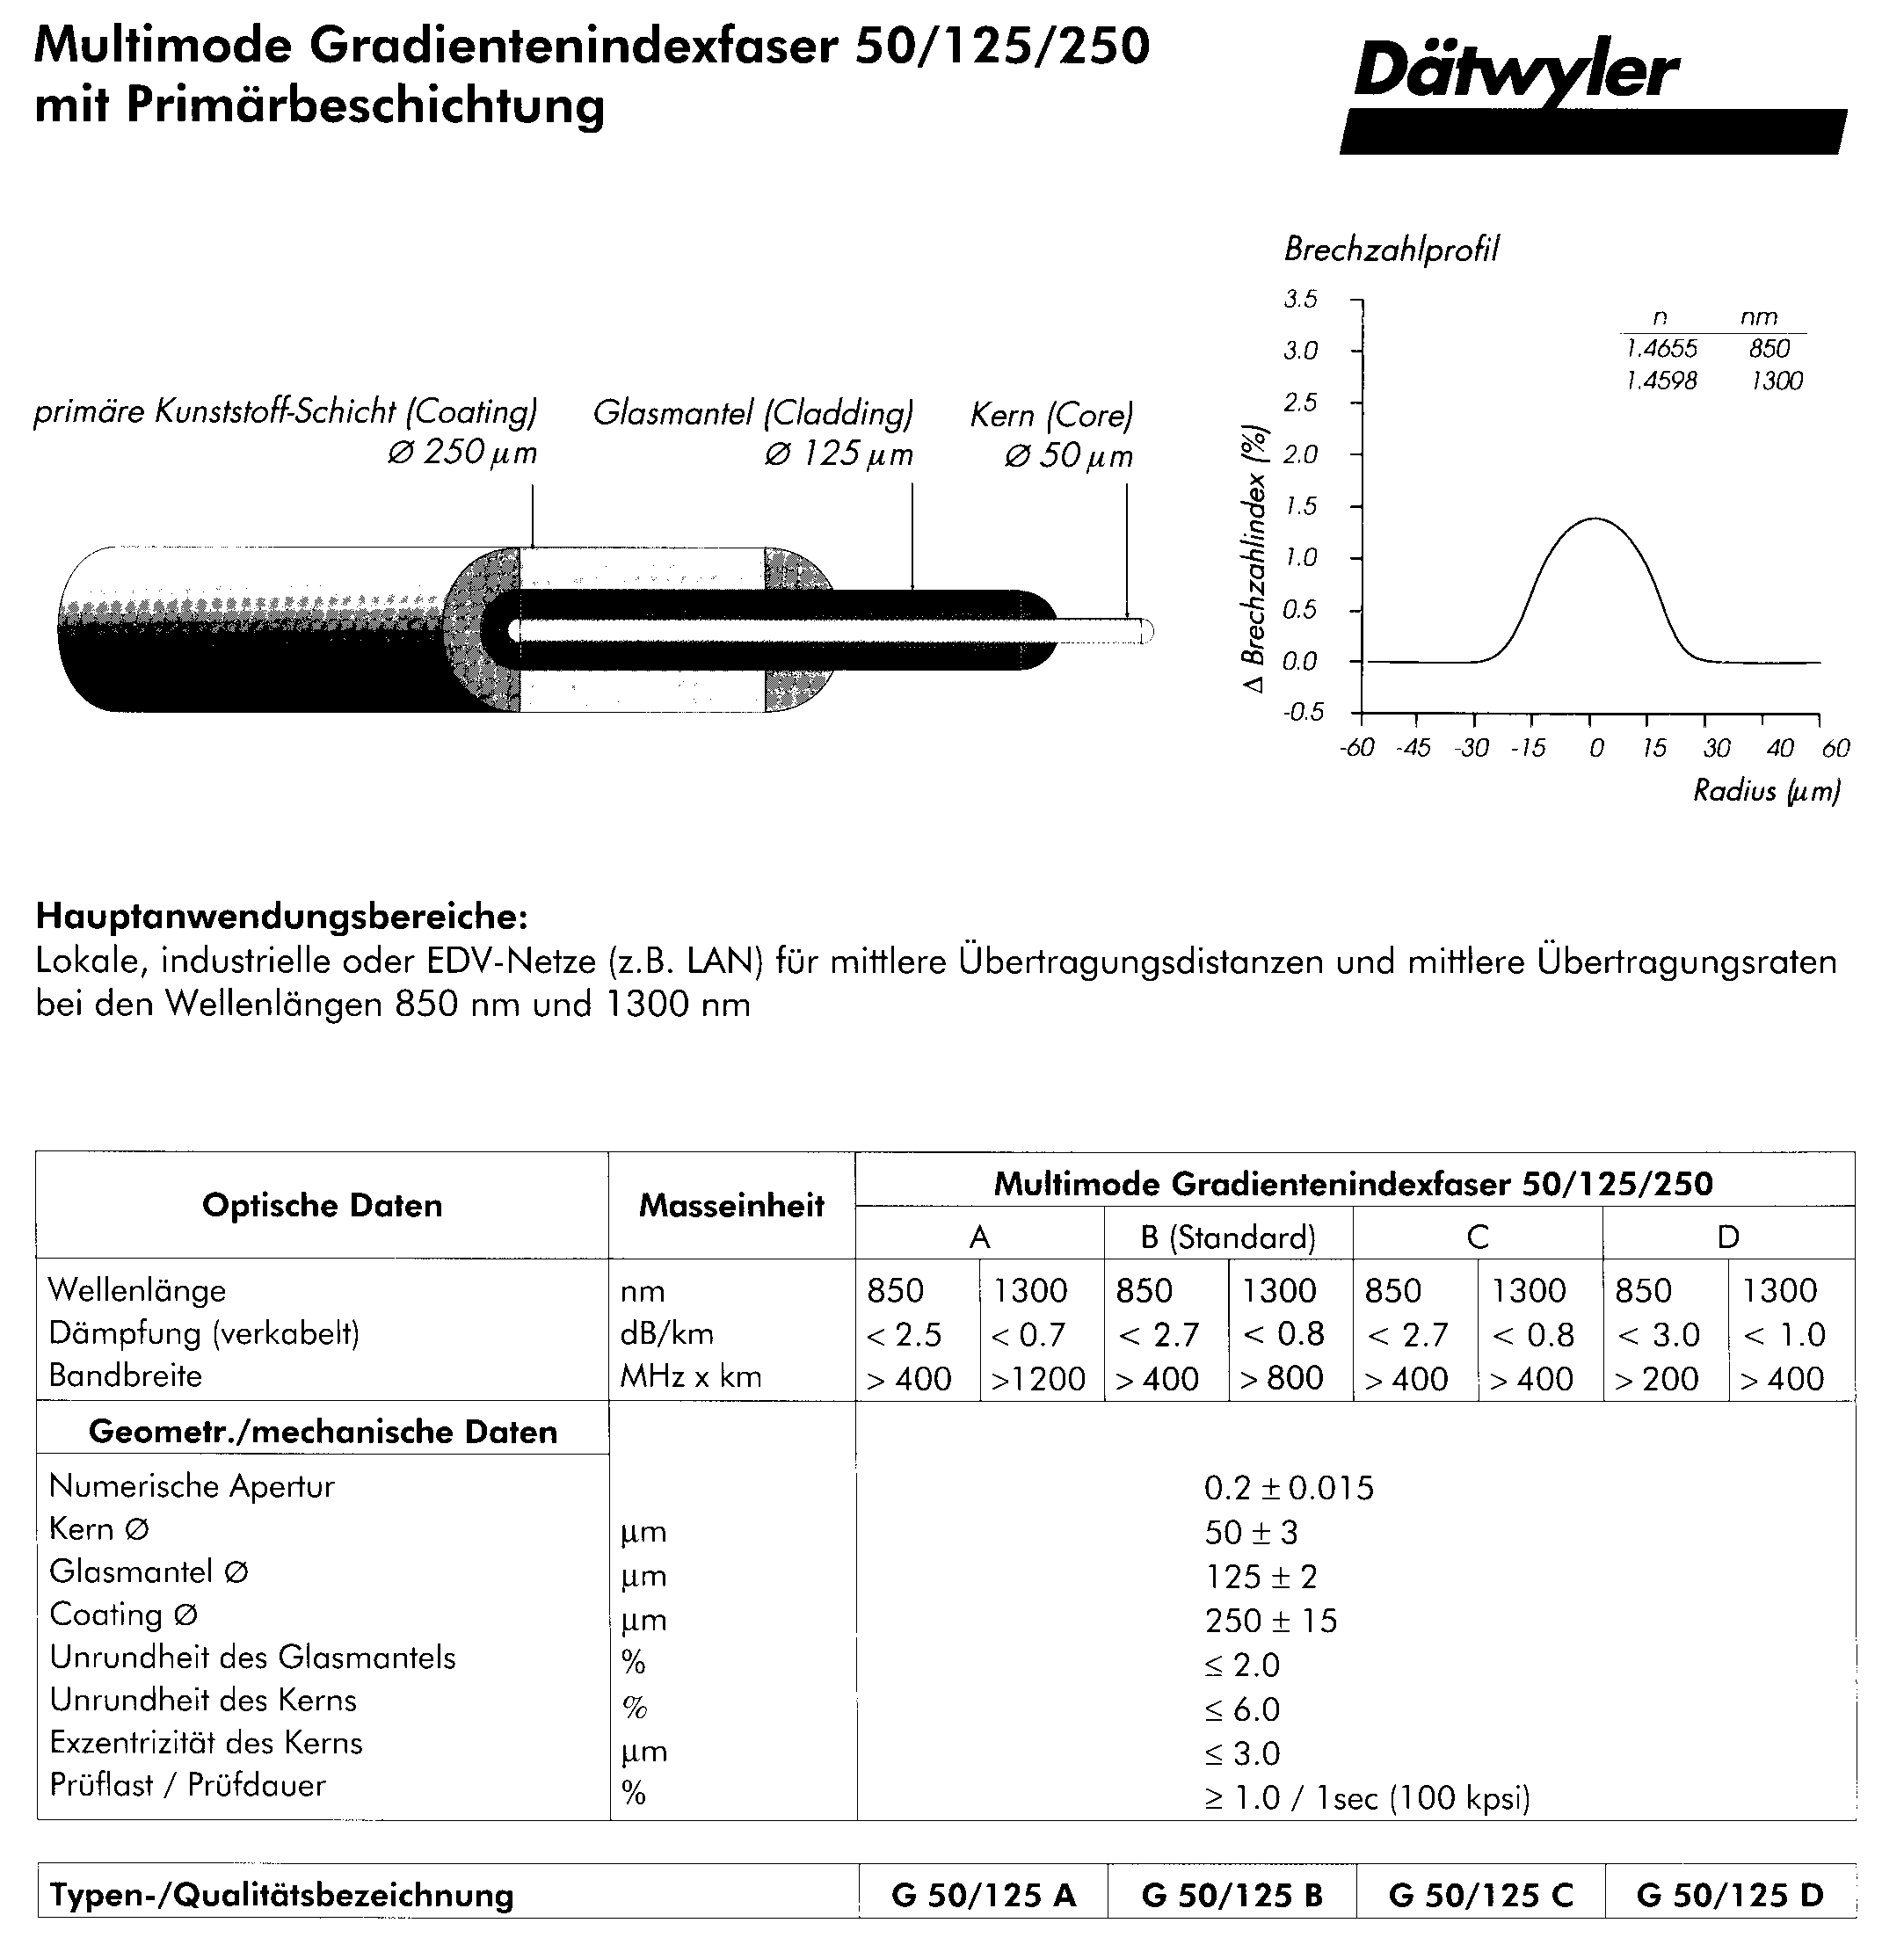
\includegraphics[width=18cm]{Library/Uebung_27-10-2012/LWL-Kabel.png}


%\nopagebreak[0] \chapter{Definition und Zielsetzung}


%\chapter{KK Woche 03}





\section{Aufgabe 2.2} 

\textbf{Spartaner Aufgabe: siehe Bl�tter: 03 - Unterlagen der Woche 3 (Skytale)}\\
Beschreibe die Entschl�sselung, die vom mit 3 Tage verschl�sseltem Krypotext zum urspr�nglichem Klartext f�hrt. Weshalb bekommt man den richtigen Klartext? Haben die Spartaner eine gute Wahl getroffen?\\
\\
\textbf{Nein}, sie haben keine gute Wahl getroffen.\\
1. 2 x Caesar Verschl�sselung mit $i_1$ und $i_2$ ist gleichbedeutend mit einer Casar-Verschl�sselung mit $i_3=i_1+i_2$.\\
\\
\\
Da der Kryptoanalytiker f�r jeden Versuch lediglich $1.5 Minuten$ ben�tigt, kann er in $3 Tagen$, was $72$ Stunden entspricht und somit $4320 Minuten$ 2880 Versuche durchf�hren.\\
1. bei Caesar gibt es 25 M�glichkeiten\\
2. bei SKYTALE gibt es 100 M�glichkeiten\\
=> $25 \cdot 100 = 2500$M�glichkeiten\\
\\
\textbf{Verschl�sselung w�rde in weniger als 3 Tagen genackt werden!!!}


\subsection{Unterkapitel 1}
%\input{Library/2-DZ}
%\input{Library/2-DZ/1-Def}
%\input{Library/2-DZ/2-HistEntw}
%\input{Library/2-DZ/3-Ziel}
%\input{Library/3-ITILv3}
%\input{Library/3-ITILv3/1-ITILv3Ovrview}
%\input{Library/4-Beispiel}
\end{normalsize}

\listoffigures
\nocite{*} 
\bibliography{bib/verzeichnis1}{}
\bibliographystyle{plain}
\end{spacing}
\end{document}